\documentclass[a4paper,12pt]{article}
\usepackage{tikz}
\usetikzlibrary{calc}
\begin{document}

%\begin{center}
%\begin{tikzpicture}
%
%	\foreach \i [remember=\i as \j (initially 0), evaluate=\i as \c using 100*\i/100] in {10,20,...,100} {
%		%\fill [yellow!\c](\j:0.5) circle (0.5);
%		\fill [red!\c](\i:1) circle (0.5);
%		%\fill [blue!\c](-\j:0.5) circle (0.5);
%		\fill [black!\c](-\i:1) circle (0.5);
%	}
%\end{tikzpicture}
%\end{center}
%\begin{figure}
%%\centering
%\begin{tikzpicture}[line width=0.8pt]
%\foreach \i in {-9,...,9}{
%	\foreach \j in {-9,...,9}{
%		\coordinate(v\i\j) at (\i,\j);
%		\foreach \k in {1,...,8}{
%			\coordinate(v\i\j\k) at ($(v\i\j)+(\k*45-22.5: 0.3)$);
%		}
%	}
%}
%
%\draw (v02)--(v04)--(v26)--(v46)node[near start, above]{$a$}--(v64)--(v62)node[near end, right]{$a^{-1}$}--(v40)--(v20)--cycle;
%
%\draw [dashed](v33)--(v11);
%\draw [dashed](v33)--(v03);
%\draw [dashed](v33)--(v15);
%\draw [dashed, ->](v33)--(v37);
%\draw [dashed](v33)--(v55);
%\draw [dashed](v33)--(v63);
%\draw [dashed, ->](v73)--(v63);
%\draw [dashed](v33)--(v51);
%\draw [dashed](v33)--(v30);
%
%\draw [dashed, ->](v33)--(v30);
%
%
%\end{tikzpicture}
%\end{figure}

\begin{figure}
\centering
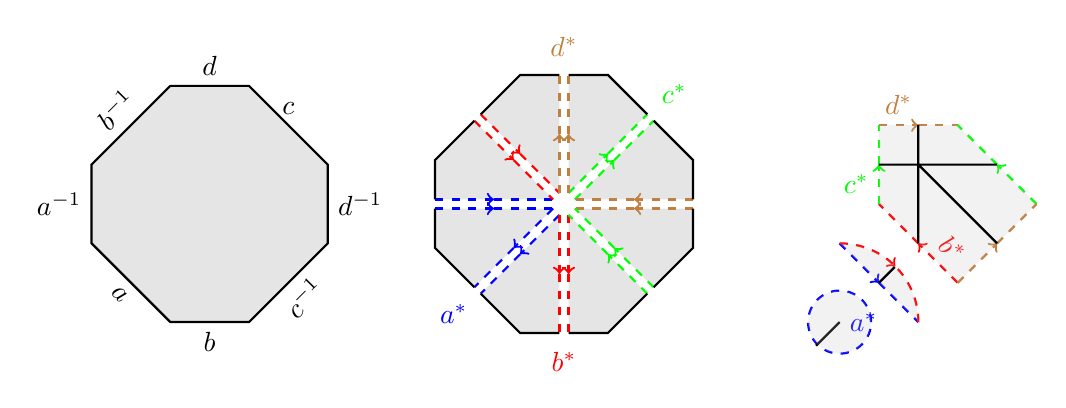
\begin{tikzpicture}[line width=0.8pt,scale=0.5]
\foreach \i in {-9,...,9}{
	\foreach \j in {-9,...,9}{
		\coordinate(v\i\j) at (\i,\j);
		\foreach \k in {1,...,8}{
			\coordinate(v\i\j\k) at ($(v\i\j)+(\k*45-22.5: 0.3)$);
		}
	}
}

\draw [fill=gray!20](v-70)--node[midway,sloped,below]{$a$}(v-92)--node[midway,left]{$a^{-1}$}(v-94)--node[midway,sloped,above]{$b^{-1}$}(v-76)--node[midway,sloped,above]{$d$}(v-56)--node[midway,above]{$c$}(v-34)--node[midway, right]{$d^{-1}$}(v-32)--node[midway,sloped, below]{$c^{-1}$}(v-50)--node[midway,sloped,below]{$b$}cycle;

%5
\fill [gray!20] (v335)--(v115)--(v025)--(v035)--cycle;
%a^*
\draw [blue, dashed, ->](v335)--(v225);
\draw [blue, dashed](v225)--(v115);
\draw [blue] (0.2,0.2)node{$a^*$};
%a^*-1
\draw [blue, dashed, ->](v035)--++(1.5,0);
\draw [blue, dashed](v035)++(1.5,0)--(v335);

\draw (v115)--(v025)--(v035);

%4
\fill [gray!20](v334)--(v034)--(v044)--(v154)--cycle;
%a^*-1
\draw [blue, dashed, ->](v034)--++(1.5,0);
\draw [blue, dashed](v034)++(1.5,0)--(v334);
%b^*-1
\draw [red, dashed, ->](v154)--(v244);
\draw [red, dashed](v244)--(v334);

\draw (v034)--(v044)--(v154);

%3
\fill [gray!20](v333)--(v153)--(v263)--(v363)--cycle;
%b^*-1
\draw [red, dashed, ->](v153)--(v243);
\draw [red, dashed](v243)--(v333);
%d^*
\draw [brown, dashed, ->](v333)--++(0,1.5);
%\draw [brown, dashed](v333)++(0,1.5)--node[midway,right]{$d^*$}(v363);
\draw [brown, dashed](v333)++(0,1.5)--(v363);
\draw [brown] (v37)node{$d^*$};

\draw (v153)--(v263)--(v363);

%2
\fill [gray!20](v332)--(v362)--(v462)--(v552)--cycle;
%c^*
\draw [green, dashed, ->](v332)--(v442);
\draw [green, dashed](v442)--(v552);

%d^*
\draw [brown, dashed, ->](v332)--++(0,1.5);
\draw [brown, dashed](v332)++(0,1.5)--(v362);

\draw (v362)--(v462)--(v552);

%1
\fill [gray!20](v331)--(v551)--(v641)--(v631)--cycle;
%c^*
\draw [green, dashed, ->](v331)--(v441);
%\draw [green, dashed](v441)--node[midway,sloped,below]{$c^*$}(v551);
\draw [green, dashed](v441)--(v551);
\draw [green] (5.8,5.8)node{$c^*$};
%d^*-1
\draw [brown, dashed, ->](v631)--++(-1.5,0);
\draw [brown, dashed](v631)++(-1.5,0)--(v331);

\draw (v551)--(v641)--(v631);

%8
\fill [gray!20](v338)--(v638)--(v628)--(v518)--cycle;
%d^*-1
\draw [brown, dashed, ->](v638)--++(-1.5,0);
\draw [brown, dashed](v638)++(-1.5,0)--(v338);
%c^*-1
\draw [green, dashed, ->](v518)--(v428);
\draw [green, dashed](v428)--(v338);

\draw (v638)--(v628)--(v518);

%7
\fill [gray!20](v337)--(v517)--(v407)--(v307)--cycle;
%b^*
\draw [red, dashed, ->](v337)--++(0,-1.5);
%\draw [red, dashed](v337)++(0,-1.5)--node[midway,right]{$(b^*)^{-1}$}(v307);
\draw [red, dashed](v337)++(0,-1.5)--(v307);
\draw[red] (v3-1)node{$b^*$};
%c^*-1
\draw [green, dashed, ->](v517)--(v427);
\draw [green, dashed](v427)--(v337);

\draw (v517)--(v407)--(v307);

%6
\fill [gray!20](v336)--(v306)--(v206)--(v116)--cycle;
%a^*-1
\draw [blue, dashed, ->](v336)--(v226);
\draw [blue, dashed](v226)--(v116);
%b^*
\draw [red, dashed, ->](v336)--++(0,-1.5);
\draw [red, dashed](v336)++(0,-1.5)--(v306);

\draw (v306)--(v206)--(v116);


%\draw [dashed, blue,->](9,0)--node[midway, above]{$a^*$}(11,0);
%\draw [dashed, red,->](9,1)--node[midway, above]{$b^*$}(11,1);
%\draw [dashed, green,->](9,2)--node[midway, above]{$c^*$}(11,2);
%\draw [dashed, brown,->](9,3)--node[midway, above]{$d^*$}(11,3);
\foreach \i in {0,...,9}{
	\foreach \j in {0,...,9}{
		\coordinate(w\i\j) at ($(v\i\j)+(10,0)$);
		\foreach \k in {1,...,8}{
			\coordinate(w\i\j\k) at ($(w\i\j)+(\k*45-22.5: 0.3)$);
		}
	}
}

% f1
\draw [dashed, blue] (w00) circle (0.8) node[right]{$a^*$};

\draw (w00)--++(-0.6, -0.6);

\fill [gray!50, opacity=0.2] (w00) circle (0.8);

%f2
\draw [dashed, blue, ->] (w02)--(w11);
\draw [dashed, blue] (w11)--(w20);
\draw [dashed, red,->] (w02) arc (90:45: 2);
\draw [dashed, red] (w20) arc (0:45: 2);
\fill [gray!50, opacity=0.2] (w20)--(w02)arc(90:0:2)--cycle;

\draw (w11)--++(0.4,0.4);

%f3
\draw [dashed, red,->] (w31)--node[midway, sloped,above]{$b^*$}(w22);
\draw [dashed, red] (w22)--(w13);

\draw[dashed, green,->] (w13)--node[midway,left]{$c^*$}(w14);
\draw[dashed,green](w14)--(w15);
\draw[dashed, brown,->] (w15)--node[midway,above]{$d^*$}(w25);
\draw[dashed,brown](w25)--(w35);

\draw [dashed, green,->] (w53)--(w44);
\draw [dashed, green] (w44)--(w35);

\draw [dashed, brown,->] (w31)--(w42);
\draw [dashed, brown] (w42)--(w53);

\fill [gray!50,opacity=0.2] (w31)--(w13)--(w15)--(w35)--(w53)--cycle;

\draw (w25)--(w24)--(w22)--(w24)--(w14)--(w24)--(w44)--(w24)--(w42);

\end{tikzpicture}
\caption{Dualizing $aa^{-1}b^{-1}dcd^{-1}c^{-1}b$ into ($a$, $ba^{-1}$, $cd^{-1}b^{-1}c^{-1}d$)}
\end{figure}

\begin{figure}
\centering
\begin{tikzpicture}

\draw (v-10)--(v-32)node[near end, sloped,below]{$c$}--(v-14)node[near start, sloped, above]{$c^{-1}$}--(v14)node[near start, above]{$a$}--(v32)node[near start, sloped, above]{$b$}--(v10)node[near start, sloped, below]{$a^{-1}$}--cycle node[near start, below]{$b^{-1}$};


\draw [dashed](v02)--(v-21);
\draw [dashed](v02)--(v-23);
\draw [dashed](v02)--(v21);
\draw [dashed](v02)--(v23);
\draw [dashed](v02)--(v00);
\draw [dashed, ->](v02)--(v05);
\draw [dashed, ->,](v40)--(v21);

\draw [dashed] (v50)--(v54)--(v94)--(v90)--cycle;
\draw [dashed] (v50) arc (180:135:2) arc (135:90:2.06);
\draw [dashed] (v50) arc (270:315:2) arc (315:360:2.06);

\draw (v61) node{$.~v_1$};
\draw (v83) node{$.~v_2$};
\end{tikzpicture}
\end{figure}



\end{document}

